\section{Application: the program through the matrix}\label{sec:application}

\subsection{Aggregate results}\label{subsec:aggregate}

The main results for applying the demand stimulus as described in Section~\ref{sec:io-bridge} to a set of model economies as conceptualized in Sections~\ref{sec:two-questions} and \ref{sec:kernel} are summarized in Table~\ref{tab:results-matrix} below. This table asks a more direct question of the fifteen cells captured in our exposition: it reports the economic valuation of the outcomes rather than the mechanics of the adjustment.

We find that the resulting matrix describes nine distinct economies rather than fifteen: the employment adjustment and Leontief columns coincide exactly, and under the three flexible-wage columns the tax-financed and the externally financed variants do so as well. Since the demand shock is identical across scenarios, the differences between the columns reflect only how the economy absorbs the program, and this absorption depends on the interaction of the labor-market and financing closures.

% =====================================================================
% Table 4 --- results across the 5x3 closure matrix (GENERATED)
% ---------------------------------------------------------------------
% Do NOT edit by hand. Regenerate with:  make_table4_results.py
% Source: runs/matrix_5x3-<closure>-<fin>/manifest.toml (schema v2);
%   elastic-supply column: the executed sectoral cells
%   matrix_5x3-BETA-<fin>-etas{05,1,2}, reported as a min--max bracket.
% Columns in table3 order (no-reallocation leftmost). Five outcomes per cell:
%   \Delta Y real GDP, \Delta L employment, \Delta\omega average real consumption
%   wage (metrics.wage; the CPI is one in every demand-only cell, ADR-0058),
%   \Delta D net external position (= F + B_gov, 'external debt'),
%   \Delta W_C household consumption welfare.
% All in percent vs. the baseline; GDP at basic prices = 1.
% COLLAPSED CELLS: F2/F3 share one cell in the three flexible-wage columns
%   (\multirow{2}, the rule between those rows is a \cmidrule over the two
%   right-hand columns only); the employment-adjustment and Leontief columns share
%   one \multicolumn{2} cell per row. The generator asserts both coincidences
%   on the printed strings, so a broken equivalence aborts the build.
% =====================================================================
\begin{table}[htbp]
\centering
\footnotesize
\setlength{\tabcolsep}{3pt}
\setlength{\parindent}{0pt}
\setlength{\parskip}{2pt}
\renewcommand{\arraystretch}{1.25}
\begin{tabular}{@{}>{\raggedright\arraybackslash}p{1.6cm} >{\raggedright\arraybackslash}p{2.1cm} >{\raggedright\arraybackslash}p{2.1cm} >{\raggedright\arraybackslash}p{3.2cm} | >{\raggedright\arraybackslash}p{2.1cm} >{\raggedright\arraybackslash}p{2.1cm}@{}}
\toprule
\textbf{Financing closure}
& \textbf{No-reallocation}\newline \scriptsize immobile labor, sectoral wages
& \textbf{Standard CGE}\newline \scriptsize one flexible wage, mobile labor
& \textbf{Elastic labor supply}\newline \scriptsize sectoral supply on the real wage\newline {\footnotesize\begin{tabular}{@{}>{\raggedright\arraybackslash}p{0.85cm}@{\hspace{3pt}}>{\raggedleft\arraybackslash}p{2.2cm}@{}}
& $\eta_s \in [0.5,2]$\end{tabular}}
& \textbf{Employment adjustment}\newline \scriptsize wage pinned, employment uncapped
& \textbf{Leontief closure}\newline \scriptsize wage pinned, quantities absorb
\\
\midrule
\textbf{F1}\newline \scriptsize repurposing of consumption
& \begin{tabular}{@{}l@{\hspace{3pt}}r@{}}
$\Delta Y$ & $-0.01$ \\
$\Delta L$ & $0.00$ \\
$\Delta\omega$ & $+0.62$ \\
$\Delta D$ & $-0.58$ \\
$\Delta W_C$ & $+0.10$\end{tabular}
& \begin{tabular}{@{}l@{\hspace{3pt}}r@{}}
$\Delta Y$ & $0.00$ \\
$\Delta L$ & $0.00$ \\
$\Delta\omega$ & $0.00$ \\
$\Delta D$ & $+0.08$ \\
$\Delta W_C$ & $+0.14$\end{tabular}
& \begin{tabular}{@{}>{\raggedright\arraybackslash}p{0.85cm}@{\hspace{3pt}}>{\raggedleft\arraybackslash}p{2.2cm}@{}}
$\Delta Y$ & $[+0.12,\ +0.19]$ \\
$\Delta L$ & $[+0.12,\ +0.19]$ \\
$\Delta\omega$ & $[+0.10,\ +0.27]$ \\
$\Delta D$ & $[-0.09,\ +0.14]$ \\
$\Delta W_C$ & $[+0.42,\ +0.58]$\end{tabular}
& \multicolumn{2}{|>{\centering\arraybackslash}p{4.35cm}}{\begin{tabular}{@{}l@{\hspace{3pt}}r@{}}
$\Delta Y$ & $-0.10$ \\
$\Delta L$ & $-0.10$ \\
$\Delta\omega$ & $0.00$ \\
$\Delta D$ & $0.00$ \\
$\Delta W_C$ & $-0.08$\end{tabular}}
\\
\cmidrule(lr){1-4}\cmidrule(lr){5-6}
\textbf{F2}\newline \scriptsize refinancing via taxes
& \multirow{7}{2.1cm}[\dimexpr\baselineskip/4\relax]{\centering \begin{tabular}{@{}l@{\hspace{3pt}}r@{}}
$\Delta Y$ & $-0.02$ \\
$\Delta L$ & $0.00$ \\
$\Delta\omega$ & $+0.70$ \\
$\Delta D$ & $-0.85$ \\
$\Delta W_C$ & $-1.98$\end{tabular}}
& \multirow{7}{2.1cm}[\dimexpr\baselineskip/4\relax]{\centering \begin{tabular}{@{}l@{\hspace{3pt}}r@{}}
$\Delta Y$ & $0.00$ \\
$\Delta L$ & $0.00$ \\
$\Delta\omega$ & $0.00$ \\
$\Delta D$ & $-0.10$ \\
$\Delta W_C$ & $-1.82$\end{tabular}}
& \multirow{7}{3.2cm}[\dimexpr\baselineskip/4\relax]{\centering \begin{tabular}{@{}>{\raggedright\arraybackslash}p{0.85cm}@{\hspace{3pt}}>{\raggedleft\arraybackslash}p{2.2cm}@{}}
$\Delta Y$ & $[+0.13,\ +0.19]$ \\
$\Delta L$ & $[+0.13,\ +0.19]$ \\
$\Delta\omega$ & $[+0.11,\ +0.29]$ \\
$\Delta D$ & $[-0.28,\ -0.05]$ \\
$\Delta W_C$ & $[-1.57,\ -1.39]$\end{tabular}}
& \multicolumn{2}{|>{\centering\arraybackslash}p{4.35cm}}{\begin{tabular}{@{}l@{\hspace{3pt}}r@{}}
$\Delta Y$ & $+0.13$ \\
$\Delta L$ & $+0.13$ \\
$\Delta\omega$ & $0.00$ \\
$\Delta D$ & $0.00$ \\
$\Delta W_C$ & $-1.53$\end{tabular}}
\\
\cmidrule(lr){5-6}
\textbf{F3}\newline \scriptsize external finance
& & & & \multicolumn{2}{|>{\centering\arraybackslash}p{4.35cm}}{\begin{tabular}{@{}l@{\hspace{3pt}}r@{}}
$\Delta Y$ & $+1.78$ \\
$\Delta L$ & $+1.78$ \\
$\Delta\omega$ & $0.00$ \\
$\Delta D$ & $+1.33$ \\
$\Delta W_C$ & $+2.26$\end{tabular}}
\\
\bottomrule
\end{tabular}
\caption{Estimated impacts of a transformational stimulus in the German residential
sector across the closure matrix. Each cell reports the change in real GDP
($\Delta Y$), employment ($\Delta L$, the composite primary-factor input,
i.e.\ all value added), the average real consumption wage ($\Delta\omega$, the employment-weighted money wage deflated by the consumer price index, which equals one in every cell of this demand-only design),
the net external position ($\Delta D$, in percentage points of baseline GDP) and household consumption welfare
($\Delta W_C$), all other entries in percent against the baseline. The employment-adjustment and
Leontief columns coincide. Within each of the three flexible-wage columns, F2 and F3
coincide because the external transfer $F$ offsets the financing difference; the wage-pinned
columns impose $F=0$. The fifteen cells therefore characterize nine distinct economies.}
\label{tab:results-matrix}
\end{table}


We observe that the overall output response to the demand shock is strongly influenced by the choice of financial closure in the fixed wage models, while it is close to zero for the core neoclassical models in the two leftmost columns. As already indicated, out of these two only the no-reallocation is able to generate price reactions for the simple one-factor model under consideration, visible in Table~\ref{tab:results-matrix} through its real-wage response ($\Delta\omega$ of $+0.62\%$ and $+0.70\%$), which implies that mean wages rise faster (whereas consumer prices stay unchanged by construction). Finally, we also observe the exact neutrality of the standard CGE column, which is a property of a demand-only shock under constant returns. 

The response of GDP in the elastic labor supply column also remains marginal relative to the size of the stimulus ($+0.12\%$ to $+0.19\%$ vs. $+1.33\%$ in stimulus size), but still paints a slightly more flexible picture of labor market conditions.\footnote{Because the elastic-supply responses are monotone in $\eta_s$ --- output, employment and consumption rise with it while the real-wage response and the price dispersion fall --- we report that column as an interval rather than at a single elasticity. Table~\ref{tab:sectoral} of Appendix~\ref{app:proofs} reports the full ladder of executed variants for price dispersion, employment and consumption.} However, the real wage does move in this scenario ($+0.10\%$ to $+0.29\%$), drawing in the additional labor, which, similar to the no-reallocation case, points to the capacity of sectorally differentiated models to produce price and wage changes with conventional signs out of an otherwise minimal set of assumptions. 

For the fixed wage models, recall that only under F3 is the program an addition; otherwise it repurposes existing expenditure. For F2, a Haavelmo pattern shows up on the financing side: spent taxes outweigh absorbed income in F2 relative to F1, so tax-financed spending raises GDP by $0.13\%$ on a $1.33\%$ program --- closely the measured saving rate of about $12\%$ --- and the projections stay close to the neoclassical core. External finance, by contrast, raises GDP by $1.78\%$, more than the program itself, and its welfare effect is larger still, because externally financed expenditure creates income equal to the GDP increase while higher GDP also lowers the net tax rate.

In contrast, in most of the flexible-wage cells the external transfer turns negative ($\Delta D<0$), so the economy saves abroad; the genuinely minimal effect is amplified for the no-reallocation scenario due to higher prices for exports and investment. Within each of these three columns tax financing and external finance give the same outcome, and these collapsed results are accompanied by a large drop in estimated welfare $W_C$, the \emph{T\"ornqvist welfare index} of Section~\ref{subsec:welfare}. As discussed there, the differences in $\Delta W_C$ are largely accounting mechanics, since public expenditures do not count toward it -- an assumption that will be relaxed in the next step.

While GDP estimates are typically of greater interest in applied transformation research -- exactly because they avoid the additional complexities of valuation imposed by specific welfare measures -- employing such measures can be helpful to make certain normative assumptions explicit. As scenarios of an economic repurposing or stimulus in the spirit of a socio-ecological transformation partially invite consideration of such questions, e.g.\ on shifting preferences or the welfare impact of public spending, we indicate here how welfare statements depend on further modeling choices.

To this end Table~\ref{tab:welfare-comparison} below reweighs the economic outcomes shown in different scenarios according to a greater variety of welfare measures, starting from a reproduction of the T\"ornqvist $W_C$ in the first row of each cell. This measure is then complemented first by $W_D$ which explicitly adds public demand --- the government purchases and the investment program --- to the relevant consumption basket to signify the fact that private actors are the final recipients of said expenditures. Moving to this measure rectifies large parts of the gap between changes in welfare and GDP across financing closures. Given the nature of transformational policy proposals involving such repurposing or stimulus $W_D$ is arguably a more valid candidate for welfare assessment, at least when assuming that citizens share some pro-environmental preferences.

In addition to that Table~\ref{tab:welfare-comparison} shows several measures taking the explicit CES-specifications of the utility functions into account, evaluated at the reference substitution elasticity $\sigma=0.9$ in every cell (Section~\ref{subsec:optimization}). The first one of these $W_{CES}$ rationalizes the new bundle of final demand -- that is, consumption plus the spending program as already in $W_D$ -- in terms of the preferences associated with the original bundle. The change here captures the welfare impact if we assume that the existing optimal allocation of consumer spending is disturbed by the stimulus (or the repurposing) and, hence, induces a welfare loss due to a mis-alignment between final consumption and preferences of private actors. This is also the reason why $W_{CES}$ gives comparatively skeptical evaluations of the program across the board.

The alternative specification shown, $W_{CES^*}$, in contrast assumes that the associated repurposing of spending is actually embraced by the population and that the new equilibrium is internalized. Such an assumption would come quite naturally for all scenarios with financing closure F1, which literally models a repurposing of spending by private actors. And while it may seem less intuitive for the other scenarios at first sight, there is some empirical support for the claim that some public effort is required to enable citizens to live up to their pro-environmental preferences \citep{Wissen.2021,Braganza.2025} that could substantiate such a modeling choice. In formal terms, we define $W_{CES^*}$ to value the change in the bundle (with public demand $g^{G}+g$ subsumed into the private part) at the household's updated preferences.

% =====================================================================
% Table 5 --- welfare comparison across the closure matrix (GENERATED)
% Sources: runs/matrix_5x3-<labor>-<financing>[-etas{05,1,2}]/manifest.toml
% Verification kernel: OpenCGE 1.0.0; source design, inputs, kernel-tree consistency and all recorded metrics checked.
% ---------------------------------------------------------------------
% Do NOT edit by hand. Regenerate with:
%   julia --project=. experiments/make_table5_welfare.jl
% Layout adopts the COLLAPSING ROUTINE of table4_results-5x3.tex: the two
%   coincidences the table states are PRINTED ONCE -- F2/F3 share one cell in
%   the three flexible-wage columns (\multirow, centred across the two rows,
%   the rule between them a \cmidrule over the GAMMA/DELTA pair only) and the
%   employment-adjustment and Leontief columns share one \multicolumn{2} cell per
%   row. check_collapses() asserts both on the PRINTED strings, so a broken
%   equivalence aborts the run. Column widths and the cell contents are Table
%   5's own; only the collapse/centre/rule grammar is Table 4's.
% W_C is the manifest field; W_D, W_CES and W_CES* are computed here and
%   gated against runs/<id>/manifest.toml (consumption_rel, tol 1e-6). No run
%   directory is created or modified, and no number is hand-typed.
% =====================================================================
\begin{table}[htbp]
\centering
\footnotesize
\setlength{\tabcolsep}{3pt}
\setlength{\parindent}{0pt}
\setlength{\parskip}{2pt}
\renewcommand{\arraystretch}{1.25}
\begin{tabular}{@{}>{\raggedright\arraybackslash}p{1.6cm} >{\raggedright\arraybackslash}p{2.0cm} >{\raggedright\arraybackslash}p{2.0cm} >{\raggedright\arraybackslash}p{3.5cm} | >{\raggedright\arraybackslash}p{2.0cm} >{\raggedright\arraybackslash}p{2.0cm}@{}}
\toprule
\textbf{Financing closure}
& \textbf{No-reallocation}\newline \scriptsize immobile labor, sectoral wages
& \textbf{Standard CGE}\newline \scriptsize one flexible wage, mobile labor
& \textbf{Elastic labor supply}\newline \scriptsize sectoral supply on the real wage\newline {\footnotesize\begin{tabular}{@{}>{\raggedright\arraybackslash}p{1.05cm}@{\hspace{3pt}}>{\raggedleft\arraybackslash}p{2.2cm}@{}}
& $\eta_s \in [0.5,2]$\end{tabular}}
& \textbf{Employment adjustment}\newline \scriptsize wage pinned, employment uncapped
& \textbf{Leontief closure}\newline \scriptsize wage pinned, quantities absorb
\\
\midrule
\textbf{F1}\newline \scriptsize repurposing of consumption
& \begin{tabular}{@{}l@{\hspace{3pt}}r@{}}
$W_C$ & $+0.10$ \\
$W_D$ & $-0.01$ \\
$W_{CES}$ & $-0.25$ \\
$W_{CES^*}$ & $+0.42$ \\
$W_{L}$ & $+0.42$ \\\end{tabular}& \begin{tabular}{@{}l@{\hspace{3pt}}r@{}}
$W_C$ & $+0.14$ \\
$W_D$ & $+0.08$ \\
$W_{CES}$ & $-0.28$ \\
$W_{CES^*}$ & $+0.53$ \\
$W_{L}$ & $+0.53$ \\\end{tabular}& \begin{tabular}{@{}>{\raggedright\arraybackslash}p{1.05cm}@{\hspace{3pt}}>{\raggedleft\arraybackslash}p{2.2cm}@{}}
$W_C$ & $+0.42$--$+0.58$ \\
$W_D$ & $+0.26$--$+0.40$ \\
$W_{CES}$ & $-0.04$--$+0.06$ \\
$W_{CES^*}$ & $+0.71$--$+0.85$ \\
$W_{L}$ & $+0.58$--$+0.64$ \\\end{tabular}& \multicolumn{2}{|>{\centering\arraybackslash}p{4.05cm}}{\begin{tabular}{@{}l@{\hspace{3pt}}r@{}}
$W_C$ & $-0.08$ \\
$W_D$ & $-0.09$ \\
$W_{CES}$ & $-0.45$ \\
$W_{CES^*}$ & $+0.35$ \\
$W_{L}$ & $+0.46$ \\\end{tabular}}\\
\cmidrule(lr){1-4}\cmidrule(lr){5-6}
\textbf{F2}\newline \scriptsize refinancing via taxes
& \multirow{7}{2.0cm}[\dimexpr\baselineskip/4\relax]{\centering \begin{tabular}{@{}l@{\hspace{3pt}}r@{}}
$W_C$ & $-1.98$ \\
$W_D$ & $-0.03$ \\
$W_{CES}$ & $-0.32$ \\
$W_{CES^*}$ & $+0.51$ \\
$W_{L}$ & $+0.51$ \\\end{tabular}}& \multirow{7}{2.0cm}[\dimexpr\baselineskip/4\relax]{\centering \begin{tabular}{@{}l@{\hspace{3pt}}r@{}}
$W_C$ & $-1.82$ \\
$W_D$ & $+0.08$ \\
$W_{CES}$ & $-0.29$ \\
$W_{CES^*}$ & $+0.54$ \\
$W_{L}$ & $+0.54$ \\\end{tabular}}& \multirow{7}{3.5cm}[\dimexpr\baselineskip/4\relax]{\centering \begin{tabular}{@{}>{\raggedright\arraybackslash}p{1.05cm}@{\hspace{3pt}}>{\raggedleft\arraybackslash}p{2.2cm}@{}}
$W_C$ & $-1.57$--$-1.39$ \\
$W_D$ & $+0.27$--$+0.41$ \\
$W_{CES}$ & $-0.06$--$+0.05$ \\
$W_{CES^*}$ & $+0.77$--$+0.88$ \\
$W_{L}$ & $+0.63$--$+0.67$ \\\end{tabular}}& \multicolumn{2}{|>{\centering\arraybackslash}p{4.05cm}}{\begin{tabular}{@{}l@{\hspace{3pt}}r@{}}
$W_C$ & $-1.53$ \\
$W_D$ & $+0.30$ \\
$W_{CES}$ & $-0.07$ \\
$W_{CES^*}$ & $+0.76$ \\
$W_{L}$ & $+0.62$ \\\end{tabular}}\\
\cmidrule(lr){5-6}
\textbf{F3}\newline \scriptsize external finance
& & & & \multicolumn{2}{|>{\centering\arraybackslash}p{4.05cm}}{\begin{tabular}{@{}l@{\hspace{3pt}}r@{}}
$W_C$ & $+2.26$ \\
$W_D$ & $+3.20$ \\
$W_{CES}$ & $+2.83$ \\
$W_{CES^*}$ & $+3.66$ \\
$W_{L}$ & $+1.70$ \\\end{tabular}}\\
\bottomrule
\end{tabular}
\caption{Welfare comparison across different closures in the closure matrix.
The variables reported in each cell are welfare estimates of an identical
allocation, all in percent against the baseline. $W_C$ is the
household-consumption index of Table~\ref{tab:results-matrix}; $W_D$ the
quantity index of demand over $c^{h}+g^{G}+g$;
$W_{CES}$ the CES evaluation of the change in that bundle at the \emph{baseline}
tastes (public demand included, both bundles valued at the dated preferences);
$W_{CES^*}$ the same comparison at the household's \emph{adopted} (post-program)
tastes. $W_{L}$ the leisure-augmented form, also charging the program's extra work
hours.}
\label{tab:welfare-comparison}
\end{table}


Every measure up to this point values the bundle alone; the final row of Table~\ref{tab:welfare-comparison}, $W_L$, also charges the household for the additional primary-factor input a program requires: a gain paid for in additional hours of labor no longer counts as a free gain. The leisure cost of additional employment (or the benefit of its reduction) is extrapolated from the paid wage, with saving treated as a leakage; the remaining setup follows $W_{CES^*}$. We observe the same values for $W_L$ as we did for $W_{CES^*}$ in the first two scenarios, where employment remains effectively unchanged. For the remaining scenarios it lies mostly below $W_{CES^*}$, where the exact deviation is driven by the expansion of employment, which can lead to a strong discount on welfare gains especially for those scenarios that show the strongest expansion in employment. The inverse constellation is observed for the two fixed wage scenarios under financial closure F1, where employment slightly decreases, which leads to a welfare benefit for $W_L$ that remains unseen by $W_{CES^*}$.\footnote{The exact money-metric measure of Section~\ref{subsec:welfare} is not tabulated separately; the five indices in Table~\ref{tab:welfare-comparison} are valuation choices evaluated at one and the same allocation.}

Taken as a whole, a focus on GDP seems apt and adequate for many purposes in research aiming to connect input--output modeling and concerns for a socio-ecological transformation. However, as welfare measures are widely used and because socio-ecological transformation research addresses behavioral and normative dimensions, our short exposition served to illustrate how specific welfare measures can encode specific valuation assumptions and, correspondingly, political views and arguments. 

\subsection{Sectoral results}\label{subsec:sectoral}

The aggregate results presented in Table~\ref{tab:results-matrix} conceal how concentrated the impulse is: the program buys from only seven of the 71 sectors, and in three of them its purchases exceed $5\%$ of their baseline gross output. Figure~\ref{fig:sectoral-comparison} follows three sectors across the no-reallocation, elastic labor supply and Leontief closures: electrical equipment, which the program targets directly; metal ores and other mining, an upstream supplier; and other personal services, a consumer service the program does not buy from. For each labor closure, the bar spans the three financing closures and a line marks each financing cell. Figure~\ref{fig:sectoral-comparison-scatter} plots all 71 sectors in the output--price plane for the same three labor closures, under repurposed consumption (F1) and external financing (F3). Appendix~\ref{app:sectoral-panels} reports the full cell-by-cell panels.

\begin{figure}[htbp]
\centering
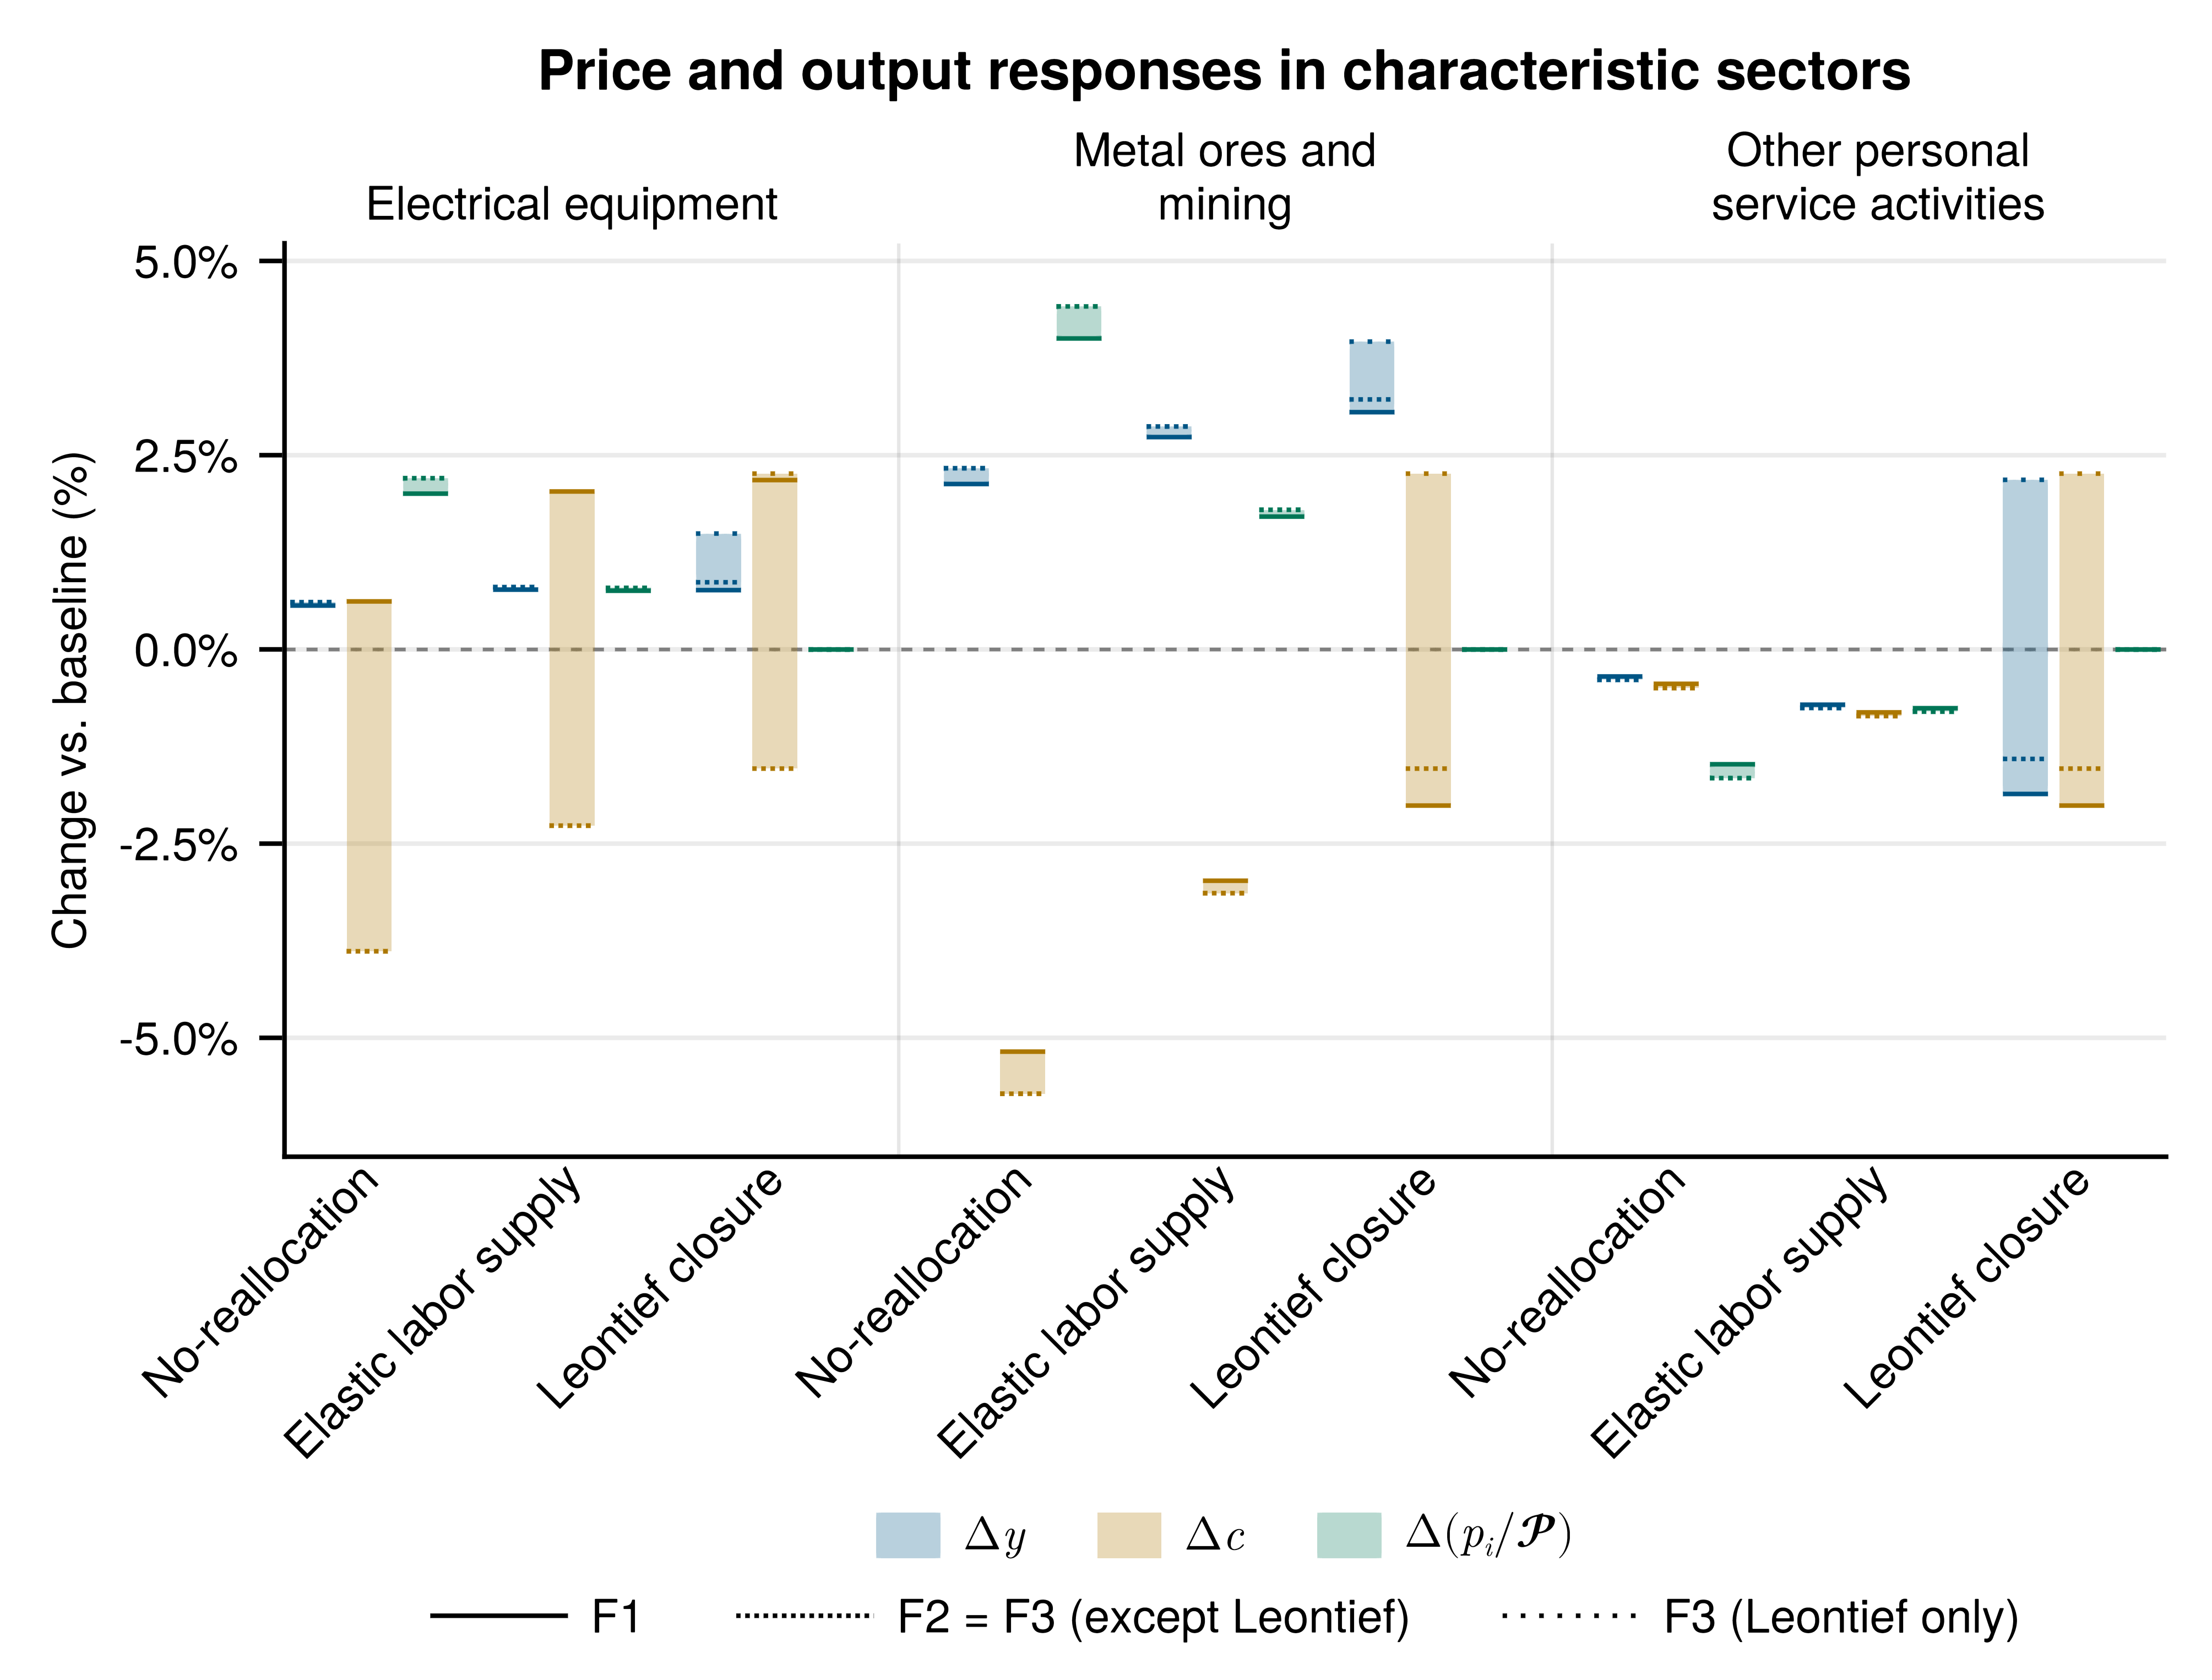
\includegraphics[width=\textwidth]{images/closure_comparison.png}
\caption{Sectoral changes in gross output ($\Delta y$), sectoral household consumption ($\Delta c^h$) and prices relative to the consumption basket ($\Delta(p_i/\mathcal{P})$) for a program sector, an upstream supplier and a consumer service, under no reallocation, elastic labor supply and the Leontief closure. Each labor group spans repurposing of consumption, tax financing and external finance; line styles identify the financing outcomes. Elastic labor supply uses $\eta_s=0.5$. Changes are relative to the no-program baseline.}
\label{fig:sectoral-comparison}
\end{figure}

\begin{figure}[htbp]
\centering
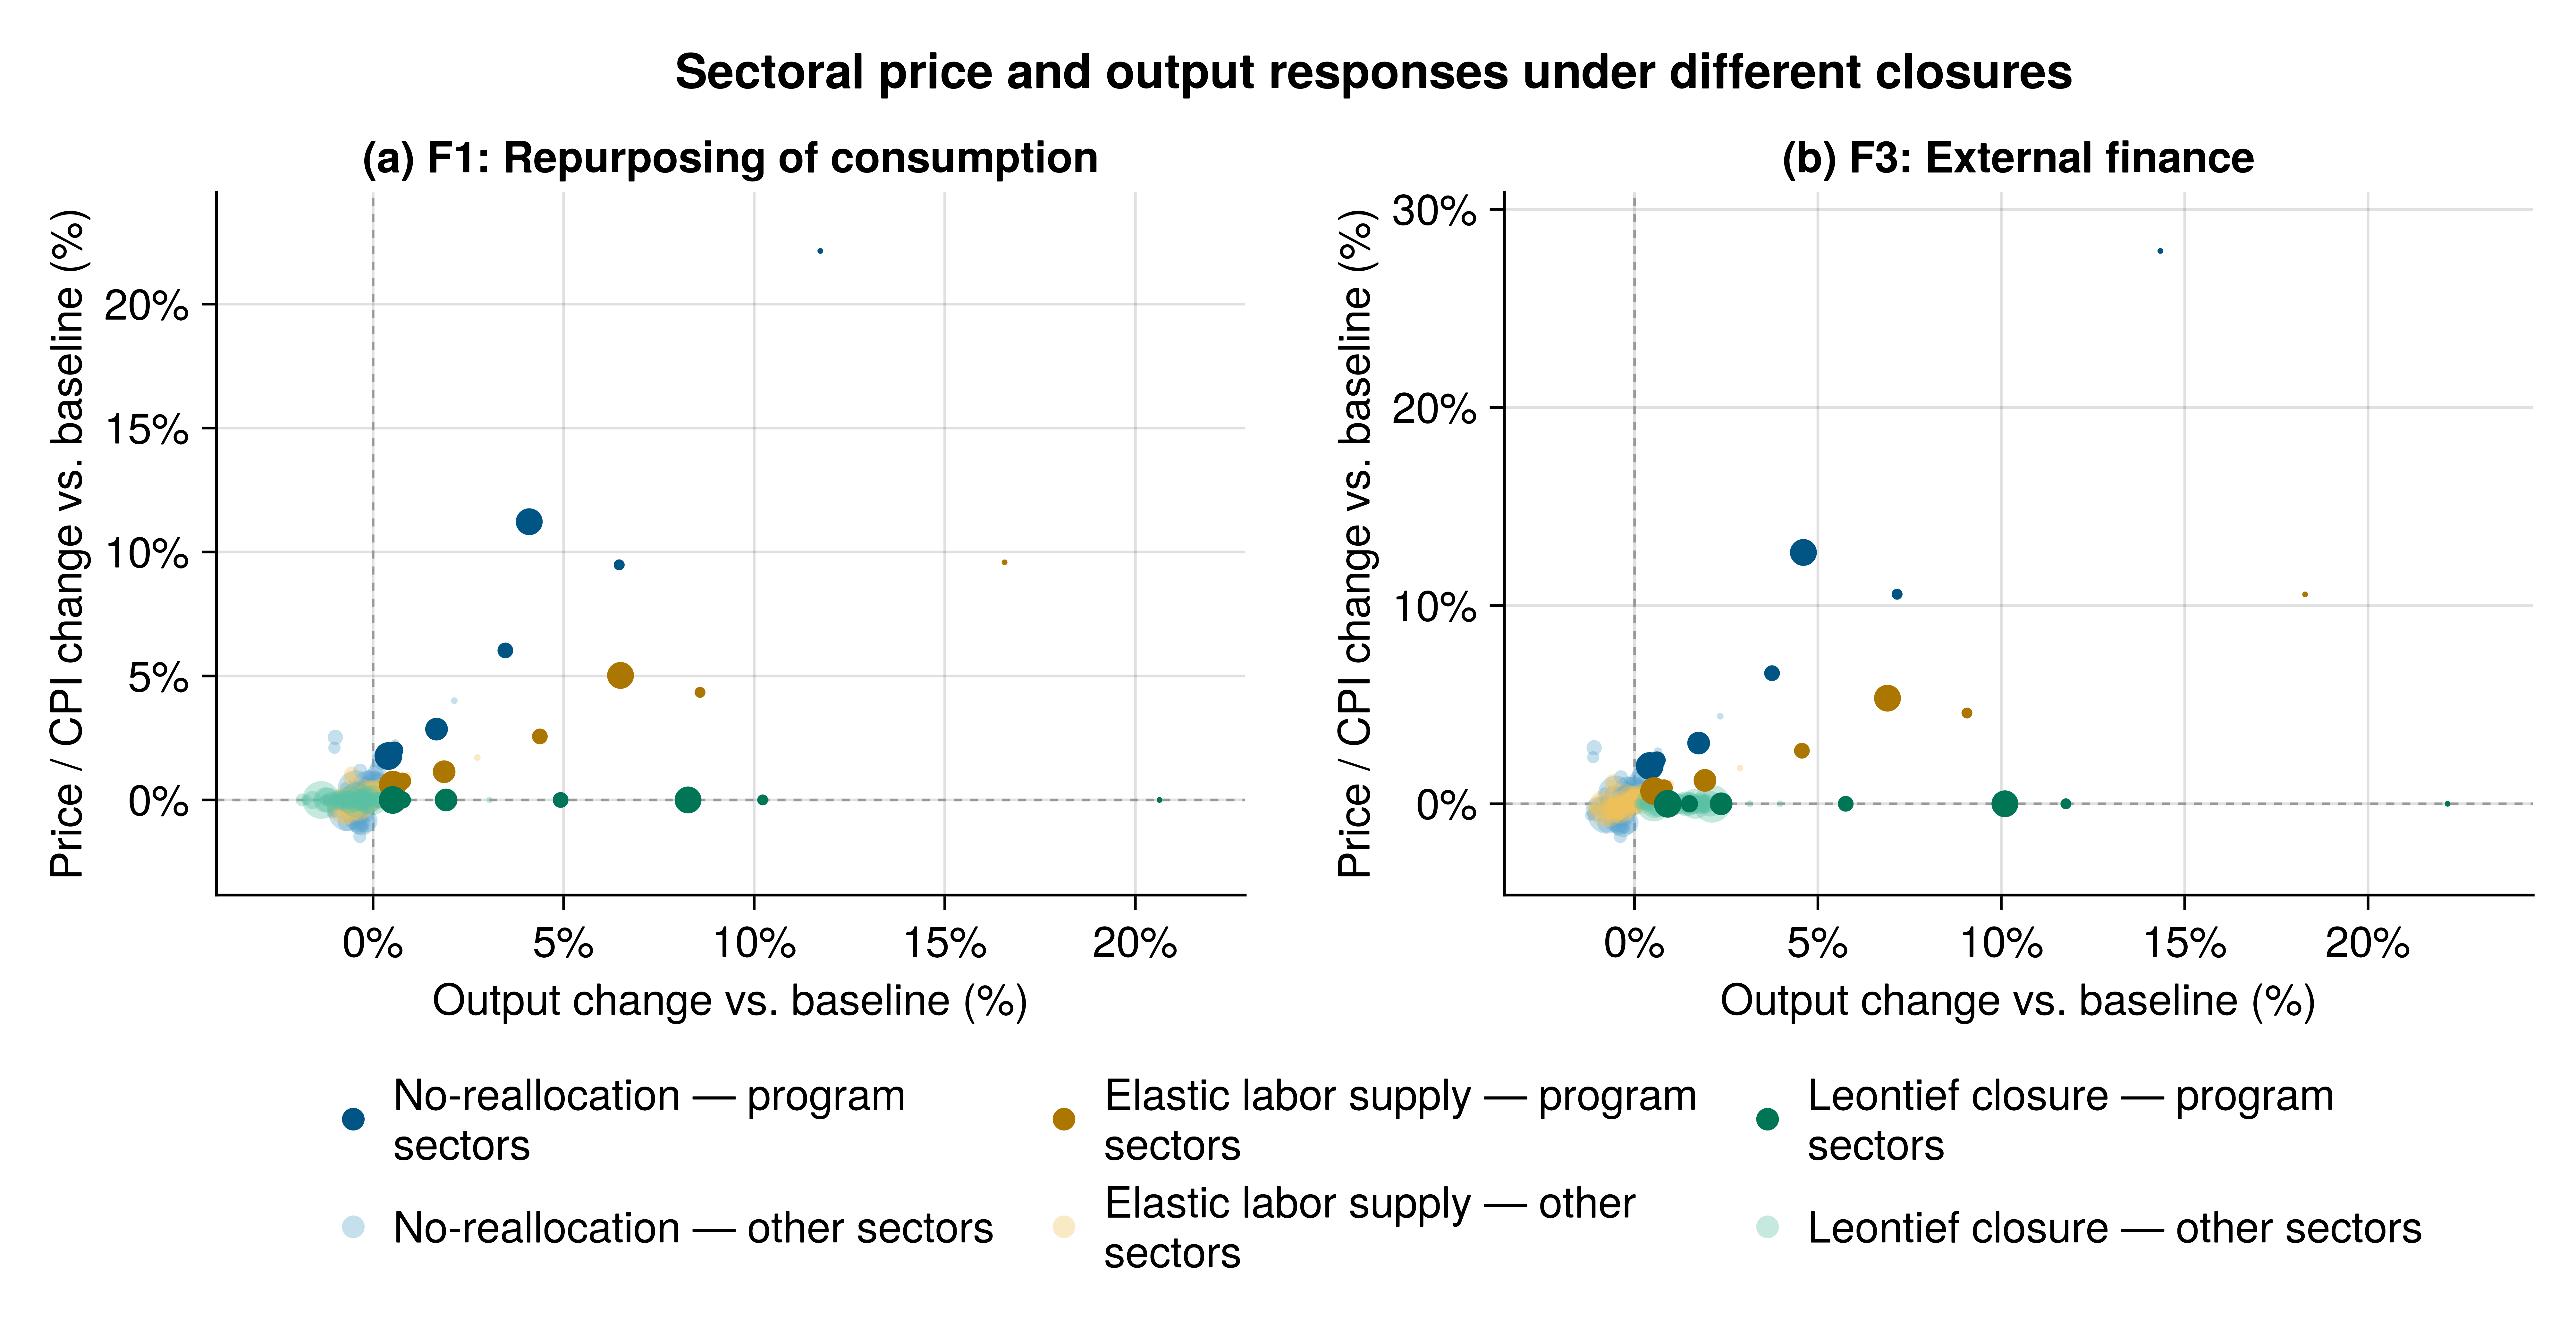
\includegraphics[width=\textwidth]{images/closure_scatter_panel.png}
\caption{Output and price changes (relative to the consumption basket) across all 71 sectors under (a) repurposing of consumption (F1) and (b) external finance (F3), comparing no reallocation, elastic labor supply ($\eta_s=0.5$) and the Leontief closure. Colors identify the labor closures and shading the program status: dark points are the seven program sectors, pale points the other sixty-four. Point area is proportional to the sector's pre-program Domar weight, i.e.\ to its gross output relative to GDP, so that a given sector carries the same area under every closure and in both panels. Each panel uses its own axis limits.}
\label{fig:sectoral-comparison-scatter}
\end{figure}

The program sectors show a similar output ranking across scenarios: glass expands most, followed by ceramics and specialized construction, while machinery and electrical equipment barely move. What the closure decides is how much of the impulse is passed through to quantities and how much is absorbed by prices. In the Leontief closure, where labor is free to move at a given wage, prices stay at the baseline and the response in sectoral output is governed by the impulse and the structure of intermediate demand: glass, for instance, expands by about 21\% on a domestic impulse of about 20\%, while ceramics expands even stronger in relative terms (about $+10.5\%$ on about $7.5\%$), because it also supplies the expanding construction sector with intermediates. Where the wage is sectoral, a part of the impulse is turned into price increases instead. In the no-reallocation column the glass sector expands by only $+11.7\%$ (F1) to $+14.3\%$ (F2/F3), while its price rises by 22\% to 28\% and its wage by more than half; elastic labor supply lies in between, with glass output up by 17\% to 18\% and its price by about 10\%. The cross-closure scatters in Figure~\ref{fig:sectoral-comparison-scatter} show that this is a systematic pattern rather than a feature of a single sector: quantities and prices move together along upward-sloping sectoral supply curves and the program sectors sit in the upper right corner.

Outside the program sectors, price changes remain small (within $\pm 1.8\%$ under elastic supply and $\pm 4.4\%$ under no-reallocation), and in each of the other eight economies a large majority of these sectors contracts: between 51 and 56 of the 64 lose output, with a median change between $-0.3\%$ and $-0.6\%$. The overall exception is the externally financed Leontief economy (Figure~\ref{fig:sectoral-comparison-scatter}(b)): here all sectors expand (with a median of $+1.4\%$ for non-program sectors), because the program adds income instead of displacing other spending and employment.

Losers are predominantly consumer-facing services, whose demand is squeezed by the reallocation of spending toward the program goods (F1) or by the taxes that finance it (F2). The few winners are upstream suppliers of the program sectors, most notably \emph{metal ores and other mining} ($+2.1\%$ to $+3.2\%$), \emph{wood products} and \emph{metal products}. In the no-reallocation column, \emph{building construction} and \emph{civil engineering} are among the strongest losers (about $-1\%$): with immobile labor they cannot share in the boom of their neighbor, specialized construction, but face its higher input prices. 




